\chapter{The \algname{} Algorithm\label{chap:approach}}

% Signposting
In this chapter, we detail \algname{}, the MaxSAT-based approach to bi-objective optimization developed in this work, together with its variants.
\Cref{sec:algorithm} gives an overview of the algorithmic framework, while \cref{sec:variants} presents five specific instantiations of one of the subroutines, based on established MaxSAT algorithms.
To conclude the chapter, in \cref{sec:refinements} we discuss refinements to \algname{}.

% BiOptSat pseudo-code
\begin{algorithm}[t]
  \caption{\algname{}: MaxSAT-based  bi-objective optimization} %\TODO{Alternatively ``enumeration of'', but then it sounds like full enumeration again.}}
  \label{alg:base-algorithm}
  \textbf{Input}: A formula $\formula$, two objectives $\Obj_\inc$ and $\Obj_\dec$. \\
  \textbf{Output}: Either a single representative for each Pareto point of $\formula$ or the full Pareto front.

  \begin{algorithmic}[1]
    \STATE $\texttt{InitSATsolver}(F)$ \label{l:init-solv} 
    \STATE $(\res, \sol) \gets \satsolver(\emptyset)$ \quad\COMMENT{Invokes the SAT solver on the formula}\label{l:sols} 
    \IF{$\res=\unsat$}
      \STATE \textbf{return} ``no solutions''
    \ENDIF
    \STATE $b_\dec \gets \infty, b_\inc \gets -1$ \label{l:bounds}
    \WHILE{$\res = \sat$} \label{l:loopstart}
      \STATE $(b_\inc, \sol) \gets \Min(b_\dec , b_\inc, \Obj_\inc(\sol))$  \quad\COMMENT{Maintains $\tot(\Obj_\inc)$ (or similar)}\label{l:minim1}
      \STATE $(b_\dec, \sol) \gets  \Simpr(b_\inc , \Obj_\dec(\sol))$  \quad\COMMENT{Builds $\tot(\Obj_\dec)$}\label{l:minim2}
      \STATE \textbf{yield} $\sol$  \quad\COMMENT{Optionally:  \textbf{yield} $\E(b_\dec, b_\inc)$}\label{ln:stage3} 
      \STATE $(\res, \sol) \gets \satsolver(\{\ov{\Obj_\dec}{b_\dec}\})$\label{l:endL}
    \ENDWHILE
  \end{algorithmic}
\end{algorithm}

\section{Overview of the Algorithm\label{sec:algorithm}}

% The framework and lexicographic method
\Cref{alg:base-algorithm} details the \algname{} framework for computing the Pareto-optimal solutions of a CNF formula $\formula$ w.r.t.\ two objectives $\Obj_\inc$ and $\Obj_\dec$.
\algname{} is an instantiation of the general lexicographic method~\autocite{survey} instantiated with a SAT solver.
To find a Pareto-optimal solution, the lexicographic method for multi-objective optimization creates multiple iterative single-objective optimization problems minimizing the objectives in order, where the latter calls are under the additional constraint to not worsen the previously minimized objectives.
Once a first Pareto-optimal solution is found, the search continues by adding a constraint that one of the objectives needs to be improved.
The lexicographic method will enumerate all Pareto-optimal solutions in monotonically increasing order of the first objective.
Following \cref{obs:biobjective}, for bi-objective optimization, this means that the solutions are in decreasing order for the second objective.
For this reason, we call objective $\Obj_\inc$ \emph{increasing} and $\Obj_\dec$ \emph{decreasing}.

% Single SAT solver and high-level overview
In \algname{}, the lexicographic method is instantiated with a single SAT solver that all subroutines make use of.
This single solver instantiation is invoked incrementally and preserved (i.e., not reset) during the whole search. 
\algname{} maintains the bounds $b_\inc$ and $b_\dec$ on the two objectives $\Obj_\inc$ and $\Obj_\dec$, respectively.
In each iteration, the \Min{} procedure sets the value of $b_\inc$ to the smallest value for which there is a still-undiscovered Pareto-optimal solution $\sol^o$ for which $\Obj_\inc(\sol^o) = b_\inc$.
The value of $b_\dec$ is then set to $\Obj_\dec(\sol^o)$ by the $\Simpr$ procedure.
In the default configuration shown in \cref{alg:base-algorithm}, \algname{} solves the task of finding a single representative per Pareto point.
In case one wishes to enumerate all Pareto-optimal solutions, the \E{} procedure enumerates all Pareto-optimal solutions $\sol^o$ for which $\Obj_\inc(\sol^o) = b_\inc$ and $\Obj_\dec(\sol^o) = b_\dec$.
We note that finding a single Pareto-optimal solution can simply be done by terminating the algorithm as soon as the first Pareto-optimal solution is returned.
This first solution will also be lexicographically optimal with the increasing objective having higher priority.

% Initializing the algorithm
In detail, given a formula $\formula$ and two objectives $\Obj_\inc$ and $\Obj_\dec$, the search of \algname{} in \cref{alg:base-algorithm} starts by initializing a SAT solver with all clauses in $\formula$ on \cref{l:init-solv}.
Satisfiability (i.e., the existence of any Pareto-optimal solutions) is checked by invoking the SAT solver on its internal formula without assumptions via the $\satsolver(\emptyset)$ function (\cref{l:sols}).
Here, $\satsolver(\assumps)$ denotes an incremental invocation of the SAT solver initialized on \cref{l:init-solv}, with the set of assumptions $\assumps$.
It has three return parameters, $(\res,\sol,\core)$ where the first is either \sat{} or \unsat{}, indicating if the internal formula is satisfiable with the given assumptions.
If $\res=\sat$, $\sol$ is populated by a satisfying assignment and $\core$ is not modified;
if $\res=\unsat$, $\core$ is populated with an unsatisfiable core and $\sol$ is not modified.
In case the returned core of a specific call is not used, we will omit it as a return parameter.
On \cref{l:sols}, if $\res$ is \unsat{}, the formula has no Pareto-optimal solutions and the algorithm terminates.
Otherwise, $\sol$ is an assignment that satisfies the formula.
Before the main enumeration procedure starts, the bounds $b_\inc$ and $b_\dec$ on $\Obj_\inc$ and $\Obj_\dec$ are set to $-1$ and $\infty$, respectively.

% Main loop: minimization of increasing objective
The main search loop (\crefrange{l:loopstart}{l:endL}) iterates as long as there are Pareto-optimal solutions of $\formula$ that have not been enumerated yet. 
This is the case if there is a solution $\sol$ for which $\Obj_\dec(\sol) < b_\dec$, checked by invoking the SAT solver under the assumption $\ov{\Obj_\dec}{b_\dec}$ on \cref{l:endL}.
In the beginning of each main loop iteration, the procedure $\Min$ is employed to minimize the increasing objective, i.e., to compute the smallest value $b_\inc$ for which there is a solution $\sol^m$ with $\Obj_\inc(\sol^m) = b_\inc$ and $\Obj_\dec(\sol^m) < b_\dec$ (\cref{l:minim1}). 
The parameters of the $\Min$ procedure are the bound $b_\dec$ that the decreasing objective of the found solution needs to be below, $b_\inc$ as a known lower and $\Obj_\inc(\tau^r)$ as a known upper bound on the minimum increasing objective value.
We assume that $\Min$ maintains a way to enforce that $\Obj_\inc(\sol) < b$, e.g., through a totalizer $\tot(\Obj_\inc)$, and that \algname{} and all of its subroutines have access to a set of assumptions for enforcing this bound for any $b$.
Details of different instantiations of the \Min{} subroutine are discussed in \cref{sec:variants}.

% Main loop: minimization of decreasing objective
Next, the algorithm employs \emph{solution-improving search}~\autocites{handbook2-maxsat,DBLP:journals/jsat/BerreP10,DBLP:journals/jsat/EenS06} to minimize the decreasing objective, i.e., to compute the smallest $b_\dec$ for which there is a solution $\sol^o$ with $\Obj_\inc(\sol^o) = b_\inc$ and $\Obj_\dec(\sol^o) = b_\dec$ (\cref{l:minim2}).
The totalizer $\tot(\Obj_\dec, \Obj_\dec(\sol))$ is built the first time this subroutine is invoked.
Building the totalizer at this point allows for only building it up to bound $\Obj_\dec(\sol)$, since all Pareto-optimal solutions are known to have at most that value for $\Obj_\dec$.
Solution-improving search works by---starting from the known upper bound $b=\Obj_\dec(\sol)$---iteratively invoking the SAT solver under the assumptions $\{\ov{\Obj_\dec}{b}, \ove{\Obj_\inc}{b_\inc}\}$ for decreasing values of $b$ until the solver reports \unsat{}.
As soon as unsatisfiability is reached, $\Simpr$ returns $b_\dec=b+1$ and the last satisfying solution $\sol$ for which $\Obj_\inc(\sol) = b_\inc$ and $\Obj_\dec(\sol) = b_\dec$.
At this point, we know that there is no solution of $\formula$ that dominates $\sol$, so $\sol$ is returned as Pareto-optimal on \cref{ln:stage3}.
If one wants to enumerate all solutions $\sol^o$ that correspond to the Pareto point $(b_\inc,b_\dec)$, the \E{} procedure repeatedly invokes the SAT solver with the assumptions $\{\ove{\Obj_\dec}{b_\dec}, \ove{\Obj_\inc}{b_\inc}\}$ and blocks each found solution until no more solutions are found.

% Search-trace fig
\begin{figure}
  \begin{minipage}{0.377\textwidth}
    \small
    \begin{align*}
      \formula = &\bigg\{ \texttt{As-CNF}\left(\sum_ {l \in \Obj_\inc \cup \Obj_\dec} l \geq 4 \right), \\
        &(i_1 \lor i_2), (i_2 \lor i_3), (i_2 \lor i_4) \\
        &(d_1 \lor d_2), (d_2 \lor d_3), (d_2 \lor d_4) \bigg\}, \\
      \Obj_\inc =&\{ i_1, i_2, i_3, i_4 \}, \\
      \Obj_\dec =&\{ d_1, d_2, d_3, d_4 \} 
    \end{align*}
  \end{minipage}
  \;
  \begin{minipage}{0.605\textwidth}
    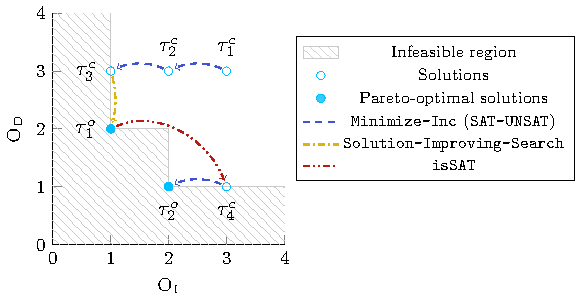
\includegraphics{search-trace.pdf}
  \end{minipage}
  \caption{Left: The same example formula $\formula$ and two objectives $\Obj_\inc$ and $\Obj_\dec$ as in \cref{fig:biobj-inst}.
    Right: the feasible region of $\formula$ in the objective space defined by $\Obj_\inc$ and $\Obj_\dec$.
    Furthermore, the search progression of the \satunsat{} variant of \algname{}.\label{fig:search-trace}}
\end{figure}

% Main algorithm example
\begin{example}\label{ex:main-iteration}
  Invoke \algname{} on the formula $\formula$ and objectives $\Obj_\inc$, $\Obj_\dec$ detailed in \cref{fig:search-trace}. 
  The search starts by invoking a SAT solver on $\formula$.
  This call returns a feasible solution, say $\sol^c_1 = \solcone$ for which $\Obj_\inc(\sol^c_1) = \Obj_\dec(\sol^c_1) = 3$. 
  The first iteration of the main search loop starts with a call to \Min{}.
  This returns $b_\inc = 1$ and, e.g., the solution $\sol^c_3 = \solcthree$ for which $\Obj_\inc(\sol^c_3) = 1$ and $\Obj_\dec(\sol^c_3) = 3$.
  \algname{} then proceeds to the \Simpr{} subroutine that initializes a totalizer $\tot(\Obj_\dec, 4)$.
  The first call to the SAT solver is made with the assumptions $\assumps = \{ \ove{\Obj_\inc}{1}, \ov{\Obj_\dec}{4} \}$.
  The result is satisfiable;
  say that the solver returns the solution $\sol^o_1 = \soloone$.
  Then, the solver is invoked with the assumptions $\assumps =  \{ \ove{\Obj_\inc}{1}, \ov{\Obj_\dec}{3} \}$.
  The result is unsatisfiable, so the procedure returns the Pareto-optimal $\sol^o_1$ and $b_\dec = \Obj_\dec(\sol^o_1) = 3$.
  Now optionally, the procedure \E{} can be used to enumerate all other solutions corresponding to the Pareto point $(\Obj_\inc(\sol^o_1),\Obj_\dec(\sol^o_1))$.
  At the end of the iteration, the SAT solver is queried with the assumption $\{ \ov{\Obj_\dec}{3} \}$.
  As the result is \sat{} and the solver returns, e.g., the solution $\sol^c_4 = \solcfour$,
  the algorithm starts a new iteration.

  The next iteration of \algname{} proceeds similarly to the first.
  The procedure \Min{} returns $b_\inc = 2$ and, e.g., the solution $\sol^o_2 = \solotwo$.
  \Simpr{} cannot improve on the decreasing objective, so the solution $\sol^o_2$ is proven to be Pareto-optimal.
  At the end of the iteration, on \cref{l:endL} the SAT solver is invoked with the assumption $\{\ov{\Obj_\dec}{2}\}$ which returns \sat{} and, e.g., the solution $\sol^o_3 = \solothree$.

  The last iteration starts by calling \Min{} which returns $b_\inc = 3$ and, e.g., again the solution $\sol^o_3$.
  \Simpr{}, again, cannot improve on the decreasing objective, so $\sol^o_3$ is also Pareto-optimal.
  Lastly, the SAT solver is queried with the assumption $\{\ov{\Obj_\dec}{1}\}$.
  The solver returns unsatisfiable, terminating the algorithm. 
\end{example}

\section{Variants for Minimizing the Increasing Objective\label{sec:variants}}

% Signposting
We consider five different instantiations of the \Min{} procedure for minimizing the increasing objective.
The first four (\satunsat{}, \unsatsat{}, \msu{} and \oll{}) are inspired by existing MaxSAT algorithms already described in \cref{sec:max-sat} while the last (\msh{}) switches between two MaxSAT-like algorithms to combine their advantages.
We do not define similar variants for the \Simpr{} procedure, since this procedure needs to perform upper-bounding search in order to be able to incrementally use the SAT solver.

\subsection{\satunsat{}\label{sec:sat-unsat}}

% SAT-UNSAT pseudo-code
\begin{algorithm}[t]
  \caption{\satunsat{} instantiation of \Min{}}\label{alg:sat-unsat}
  \textbf{Input}: Last bound $b_\dec$ on $\Obj_\dec$ and known upper bound $b$ on the minimum value of $\Obj_\inc$. \\
  \textbf{Output}: Solution $\sol$ and smallest $b=\Obj_\inc(\sol)$ so that $\Obj_\dec(\sol)<b_\dec$.

  \begin{algorithmic}[1]
    \STATE build or extend $\tot(\Obj_\inc,b)$ if necessary \label{ln:su-tot}
    \STATE $(\res,\sol) \gets \satsolver(\{\ov{\Obj_\dec}{b_\dec}, \ov{\Obj_\inc}{b}\})$
    \WHILE{$\res = \sat$}
      \STATE $b \gets \Obj_\inc(\sol)$
      \STATE $(\res,\sol) \gets \satsolver(\{\ov{\Obj_\dec}{b_\dec}, \ov{\Obj_\inc}{b}\})$ \label{ln:su-query}
    \ENDWHILE
    \STATE \textbf{return} $(b,\sol)$ \label{ln:su-ret}
  \end{algorithmic}
\end{algorithm}

% Solution-improving search and input parameters
\satunsat{} is a variant of solution-improving search~\autocites{handbook2-maxsat,DBLP:journals/jsat/BerreP10,DBLP:journals/jsat/EenS06} that is also used for minimizing $\Obj_\dec$. 
As inputs, the procedure gets the last bound $b_\dec$ on $\Obj_\dec$ and the upper bound $b=\Obj_\inc(\sol)$ on the minimum of the increasing objective known from the last SAT solver call.
The known lower bound is not needed for this variant.
Since the last call is made on \cref{l:endL} with the assumption $\ov{\Obj_\dec}{b_\dec}$, the solution $\sol$ will have $\Obj_\dec(\sol) < b_\dec$. 

% Details of SAT-UNSAT
\satunsat{} is outlined in~\cref{alg:sat-unsat}.
The procedure maintains the totalizer $\tot(\Obj_\inc)$ and begins on \cref{ln:su-tot} by checking, if the current upper bound on that totalizer is at least $b$, extending it if not. 
Then the SAT solver is iteratively invoked with the assumptions $\{\ov{\Obj_\dec}{b_\dec}, \ov{\Obj_\inc}{b}\}$ for decreasing values of $b$ (\cref{ln:su-query}).
The procedure terminates when the result is \unsat{}, after which on \cref{ln:su-ret}, the value of $b$ and the solution obtained during the final satisfiable call are returned as $b_\inc$ and $\sol$.  

% Example: SAT-UNSAT
\begin{example}\label{ex:satunsat}
  Consider the invocation of \algname{} detailed in \cref{ex:main-iteration}. 
  We detail the invocation of \Min{} instantiated as \satunsat{}. 
  The full progression of the search of \algname{} with \Min{} instantiated as \satunsat{} is illustrated in \cref{fig:search-trace}.
  In the first iteration, \satunsat{} is invoked with $b_\dec = \infty$ and $b=\Obj_\inc(\sol^c_1) = 4$.
  At this point, the totalizer over $\Obj_\inc$ has not been built, so the procedure starts by adding $\tot(\Obj_\inc, 4)$ to the solver.
  The first call to the SAT solver is made with the assumptions $\{\ov{\Obj_\inc}{4}\}$, since $b_\dec = \infty$ and therefore no assumption constraining $\Obj_\dec$ is needed.
  The result is satisfiable, the solver returns, e.g., the solution $\sol^c_2 = \solctwo$. 
  In the next iteration, the set of assumptions is $\{\ov{\Obj_\inc}{2}\}$.
  The result is again satisfiable, returning, e.g., the solution $\sol^c_3 = \solcthree$.
  The SAT solver is then invoked with the assumptions $\{\ov{\Obj_\inc}{1}\}$.
  Now the result is \unsat{} so the procedure terminates and returns $b_\inc = 1$ and $\sol^c_3$.

  In the second iteration of \algname{}, \satunsat{} is invoked with $b_\dec = 3$ and $b=\Obj_\inc(\sol^c_4) = 3$.
  The first call to the SAT solver is made with the assumptions $\{ \ov{\Obj_\dec}{3}, \ov{\Obj_\inc}{3} \}$.
  The result is \sat{} and the solver returns, e.g., the solution $\sol^o_2 = \solotwo$.
  \satunsat{} invokes the SAT solver again with the assumptions $\{ \ov{\Obj_\dec}{3}, \ov{\Obj_\inc}{2} \}$.
  The result is \unsat{}, so the procedure returns $b_\inc = 2$ and $\sol^o_2$.

  In the third (and last) iteration of \algname{}, \satunsat{} is invoked with $b_\dec = 2$ and $b=\Obj_\inc(\sol^o_3) = 3$.
  The SAT solver is queried with the assumptions $\{ \ov{\Obj_\dec}{2}, \ov{\Obj_\inc}{3} \}$ and returns \unsat{}.
  \satunsat{} therefore returns $b_\inc = 3$ and $\sol^o_3$.
\end{example}

\subsection{\unsatsat{}\label{sec:unsat-sat}}

% UNSAT-SAT pseudo-code
\begin{algorithm}[t]
  \caption{\unsatsat{} instantiation of \Min{}}\label{alg:unsat-sat}
  \textbf{Input}: Last bound $b_\dec$ on $\Obj_\dec$ and last bound $b_\inc$ on $\Obj_\inc$. \\
  \textbf{Output}: Solution $\sol$ and smallest $b=\Obj_\inc(\sol)$ so that $\Obj_\dec(\sol)<b_\dec$.

  \begin{algorithmic}[1]
    \STATE $b \gets b_\inc$ \label{ln:us-boundinit}
    \STATE build or extend $\tot(\Act,b+1)$
    \STATE $(\res,\sol) \gets \satsolver(\{\ov{\Obj_\dec}{b_\dec}, \ove{\Obj_\inc}{b+1}\})$
    \WHILE{$\res = \unsat$}
      \STATE $b \gets b+1$
      \STATE extend $\tot(\Obj_\inc,b+1)$ \label{ln:us-tot}
      \STATE $(\res,\sol) \gets \satsolver(\{\ov{\Obj_\dec}{b_\dec}, \ove{\Obj_\inc}{b+1}\})$ \label{ln:us-query}
    \ENDWHILE
    \STATE \textbf{return} $(b+1,\sol)$ \label{ln:us-ret}
  \end{algorithmic}
\end{algorithm}

% UNSAT-SAT and input parameters
\unsatsat{} takes a similar approach to \satunsat{} search but searches for the smallest value by lower-bounding instead of upper-bounding~\autocite{DBLP:conf/sat/FuM06}.
As input parameters it receives the last bound $b_\dec$ on $\Obj_\dec$ and the last bound $b_\inc$ on $\Obj_\inc$ as a lower bound on the sought-after smallest value.
The upper bound on the smallest value is not needed for this variant.
\unsatsat{} also maintains a totalizer $\tot(\Obj_\inc)$.

% Details of UNSAT-SAT
The \unsatsat{} instantiation of \Min{} proceeds as illustrated in \cref{alg:unsat-sat}.
On \cref{ln:us-boundinit}, the bound $b$ is set to the known lower bound $b_\inc$ and the solver is then iteratively queried on \cref{ln:us-query} under the assumptions $\{ \ove{\Obj_\inc}{b+1}, \ov{\Obj_\dec}{b_\dec} \}$.
If the solver returns unsatisfiable, the bound $b$ is increased by $1$ and the solver is queried again.
The search ends once the solver returns satisfiable;
in this case, the solution, and the bound are returned on \cref{ln:us-ret}.
Since the bound of this lower bounding search procedure will only monotonically increase, it is enough if the totalizer $\tot(\Obj_\inc)$ is at every step built up to the bound $b+1$ (\cref{ln:us-tot}) and extended to the next bound in the next iteration.
This way, the SAT solver is always queried over a minimum number of clauses.

% Example: UNSAT-SAT
\begin{example}
  Consider the invocation of \algname{} detailed in \cref{ex:main-iteration}. 
  Here we detail the invocation of \Min{} instantiated as \unsatsat{}.
  In the first iteration, \unsatsat{} is invoked with $b_\dec = \infty$ and $b_\inc=-1$.
  At this point, the totalizer over $\Obj_\inc$ has not been built, so the procedure starts by initializing $\tot(\Obj_\inc, 0)$ and invokes the SAT solver with the assumptions $\{\ove{\Obj_\inc}{0}\}$.
  The result is \unsat{}, so the totalizer is extended to $\tot(\Obj_\inc, 1)$ and the SAT solver invoked with the assumptions $\{ \ove{\Obj_\inc}{1}\}$.
  The result is \sat{} and the procedure returns $b_\inc = 1$ and, e.g., $\sol^c_3 = \solcthree$.

  In the second iteration of \algname{}, \unsatsat{} is invoked with $b_\dec = 3$ and $b_\inc = 1$.
  The totalizer is extended to $\tot(\Obj_\inc, 2)$ and the solver is invoked with the assumptions $\{\ove{\Obj_\inc}{2}, \ov{\Obj_\dec}{3}\}$.
  The result is \sat{}, and the routine returns $b_\inc = 2$ and, e.g., $\sol^o_2 = \solotwo$.
  
  In the last iteration of \algname{}, \unsatsat{} is invoked with $b_\dec = 2$ and $b_\inc = 2$.
  The totalizer is extended to $\tot(\Obj_\inc, 3)$ and the solver is invoked with the assumptions $\{\ove{\Obj_\inc}{3}, \ov{\Obj_\dec}{2}\}$.
  The result is \sat{}, and \unsatsat{} returns $b_\inc = 3$ and, e.g., $\sol^o_3 = \solothree$.
\end{example}

\subsection{\msu{}\label{sec:msu}}

% MSU3 pseudo-code
\begin{algorithm}[t]
  \caption{\msu{} instantiation of \Min{}}\label{alg:msu}
  \textbf{Input}: Last bound $b_\dec$ on $\Obj_\dec$ and last bound $b_\inc$ on $\Obj_\inc$. \\
  \textbf{Output}: Solution $\sol$ and smallest $b=\Obj_\inc(\sol)$ so that $\Obj_\dec(\sol)<b_\dec$.

  \begin{algorithmic}[1]
    \STATE $b \gets \max\{b_\inc,0\}$
    \STATE $(\res,\sol,\core) \gets \satsolver(\{\ov{\Obj_\dec}{b_\dec}, \ove{\Obj_\inc}{b}\} \cup \{\lnot l \mid l \in \Obj_\inc \setminus \Act\})$ \label{ln:msu-firstquery}
    \WHILE{$\res = \unsat$}
      \STATE $b \gets b+1$ \label{ln:msu-inc}
      \STATE $\core \gets \core \setminus \{\lnot\ov{\Obj_\dec}{b_\dec}, \lnot\ove{\Obj_\inc}{b}\}$
      \STATE $\Act \gets \Act \cup \core$
      \STATE build or extend $\tot(\Act,b)$ \label{ln:msu-tot}
      \STATE $(\res,\sol,\core) \gets \satsolver(\{\ov{\Obj_\dec}{b_\dec}, \ove{\Obj_\inc}{b}\} \cup \{\lnot l \mid l \in \Obj_\inc \setminus \Act\})$ \label{ln:msu-mainquery}
    \ENDWHILE
    \STATE \textbf{return} $(b,\sol)$
  \end{algorithmic}
\end{algorithm}

% MSU3 and input parameters
\msu{} implements a core-guided approach inspired by the MSU3 MaxSAT algorithm~\autocites{DBLP:journals/corr/abs-0712-1097}.
The input parameters of this subroutine are the last bound $b_\dec$ on $\Obj_\dec$ and the last bound $b_\inc$ on $\Obj_\inc$ as a lower bound on the sought-after smallest value.
The upper bound on the smallest value is not needed for this variant.

% Details of MSU3
The \msu{} instantiation does not maintain a totalizer $\tot(\Obj_\inc)$, but a set $\Act \subset \Obj_\inc$ of \emph{active} objective literals and a totalizer $\tot(\Act)$ built over them. 
Initially, $\Act = \emptyset$, i.e., all literals of $\Obj_\inc$ are inactive.
Informally speaking, an inactive literal $l \in \Obj_\inc \setminus \Act$ is assumed to the value $0$ in every invocation of the SAT solver until it is returned as part of a core.
\Cref{alg:msu} illustrates the search performed by \msu{}.
The algorithm starts from the value $b=b_\inc$ computed in the previous iteration and invokes the SAT solver with the assumptions $\assumps = \{\ove{\Act}{b}, \ov{\Obj_\dec}{b_\dec}  \} \cup \{ \lnot l \mid l \in \Obj_\inc \setminus \Act\}$ on \cref{ln:msu-firstquery}.
If the result is unsatisfiable, the SAT solver returns a core $\core \subset \{\lnot l \mid l \in \assumps\}$.
Next, the bound $b$ is increased by one, the inactive literals in $\core$ are added to $\Act$ and the totalizer $\tot(\Act)$ is extended (\crefrange{ln:msu-inc}{ln:msu-tot}).
The procedure continues until the SAT solver returns satisfiable, and a solution $\sol$ which has $\Obj_\inc(\sol) = b$ and $\Obj_\dec(\sol) < b_\dec$ is found.
At that point the value $b$ is the minimum value $\Obj_\inc(\sol)$ for any solution $\sol$ subject to $\Obj_\dec(\sol) < b_\dec$.
This is because the value of $b$ is increased monotonically, and the solver returned unsatisfiable in the second-to-last iteration. 

% Enforcing an upper bound on O_I in other places and proof of correctness
For enforcing $\Obj_\inc(\sol)\le b_\inc$ when employing \msu{}, consider an invocation of $\msu(b_\dec, b_\inc)$ made during \algname{} and assume it returns the tuple $(b_\inc, \sol)$. 
In the next call to \Simpr{}, the number of literals in $\Obj_\inc$ set to $1$ needs to be restricted to at most $b_\inc$. 
Since the totalizer maintained by \msu{} only has $\Act \subset \Obj_\inc$ as inputs, we do not have access to an output literal of form  $\ove{\Obj_\inc}{b_\inc}$.
Instead, we use  the assumptions $\{ \ove{\Act}{b_\inc}\} \cup \{ \lnot l \mid l \in \Obj_\inc \setminus \Act \}$, i.e., restrict the number of literals in $\Act$ set to $1$ to $b_\inc$ and assume the value of each inactive literal $l \in \Obj_\inc \setminus \Act$ to $0$. 
In the following proposition, we prove that doing so can be done without removing any Pareto-optimal solutions from the search. 
\begin{proposition}\label{prop:sound}
  Let $\sol^o$ be a Pareto-optimal solution of $\formula$ for which $\Obj_\inc(\sol^o) = b_\inc$.
  Then $\sol^o(l) = 0$ for all $l \in \Obj_\inc \setminus \Act$. 
\end{proposition}
\begin{proof}(Sketch)
  Since, $b_\inc$ was returned by \msu{}, we know that there exists a Pareto-optimal $\sol^o$ for which $\Obj_\inc(\sol^o) = b_\inc$ and $\Obj_\dec(\sol^o) < b_\dec$.
  By the properties of cores, we also know that \emph{any} solution $\sol^s$ of $\formula$ for which $\Obj_\dec(\sol^s) < b_\dec$ assigns at least $b_\inc$ literals in $\Act$ to $1$.
  Thus, any $\sol^n$ that assigns $\sol^n(l) = 1$ for an inactive literal $l \in \Obj_\inc \setminus \Act$ will have $\Obj_\inc(\sol^n) > b_\inc$.
\end{proof}

% Example: MSU3
\begin{example}\label{ex:msu}
  Consider the invocation of \algname{} detailed in \cref{ex:main-iteration}. 
  Here we detail the invocations of \Min{} instantiated as \msu{}. 
  In the first iteration of \algname{}, \msu{} is invoked with $b_\dec =\infty$ and $b_\inc = -1$.
  Initially, the set $\Act = \emptyset$ of active literals is empty, so the first call to the SAT solver is made with the assumptions $\assumps =  \{ \lnot i_1, \allowbreak \lnot i_2, \allowbreak \lnot i_3, \allowbreak \lnot i_4\}$.
  The result is unsatisfiable and the solver returns, e.g., $\core = \{i_1, i_2\}$. 
  The literals in $\core$ are marked as active and the totalizer $\tot(\Act, 1)$ is initialized.
  The SAT solver is then invoked with the assumptions $\assumps = \{ \lnot i_3, \lnot i_4, \ove{\Act}{1}\}$. 
  The result is satisfiable so the procedure returns, e.g., $b_\inc = 1$ and the solution $\sol^c_3 = \solcthree$.

  In the next iteration of \algname{}, \msu{} is invoked with $b_\dec = 3$ and $b_\inc = 1$.
  The set $\Act = \{i_1, i_2\}$ is kept from the previous iterations, so the first call to the SAT solver is made with the assumptions $\assumps = \{ \ov{\Obj_\dec}{3}, \allowbreak \ove{\Act}{1}, \allowbreak \lnot i_3, \allowbreak \lnot i_4 \}$.
  The result is unsatisfiable;
  assume the core returned by the solver is $\core = \{ \lnot \ov{\Obj_\dec}{3}, \allowbreak \lnot \ove{\Act}{1}, \allowbreak i_3, \allowbreak i_4 \}$.
  The totalizer outputs $\lnot \ov{\Obj_\dec}{3}$ and $\lnot \ove{\Act}{1}$ are discarded, $i_3$ and $i_4$ are added to the active literals, and the totalizer is extended to $\tot(\Act, 2)$.
  The SAT solver is queried again with the assumptions $\assumps = \{\ov{\Obj_\dec}{2}, \ove{\Act}{2}\}$;
  the result is \sat{} and the returned solution, e.g., $\sol^o_2 = \solotwo$.
  \msu{} returns $b_\inc = 2$ and $\sol^o_2$.

  In the last iteration, \msu{} is invoked with $b_\dec = 2$ and $b_\inc = 2$.
  The SAT solver is queried with the assumptions $\assumps = \{\ov{\Obj_\dec}{2}, \ove{\Act}{2}\}$.
  The result is \unsat{};
  assume the core is $\core = \{ \lnot \ov{\Obj_\dec}{2}, \lnot \ove{\Act}{2} \}$.
  Both totalizer outputs are discarded, and the totalizer is extended to $\tot(\Act, 3)$.
  The solver is queried again with the assumptions $\assumps = \{\ov{\Obj_\dec}{2}, \ove{\Act}{3}\}$.
  The result is \sat{};
  assume the returned solution is $\sol^o_3 = \solothree$.
  \msu{} returns $b_\inc = 3$ and $\sol^o_3$.
\end{example}

\subsection{\oll{}\label{sec:oll}}

% High-level OLL
As mentioned in \cref{sec:max-sat}, the OLL MaxSAT algorithm~\autocite{DBLP:conf/cp/MorgadoDM14,DBLP:journals/jsat/IgnatievMM19} builds a cardinality constraint for each core extracted from the formula, treating the totalizer outputs as part of the objective.
The same holds for the \oll{} instantiation of \Min{}.
Assume in the $i$th iteration, \oll{} extracts the core $\core_i$.
It will build a totalizer $\tot(\core_i, 1)$ and enforce $\sum_{l\in\core_i} l \le 1$ as an assumption.
For all literals in the extracted core, if the literal is part of the objective, the literal is marked as active.
If the literal is the output of a totalizer built over a previous core, the bound enforced on that totalizer is increased by one.
In each iteration, the assumptions given to the SAT solver consist of (i)~the inactive literals of $\Obj_\inc$, (ii)~the outputs of previously built totalizers corresponding to the lowest number of input literals that should be assigned to $1$ in any possible satisfying assignment, and (iii)~the bound $\ov{\Obj_\dec}{b_\dec}$.
The procedure terminates when the SAT solver returns a solution $\sol$.

Similarly to \msu{}, the assumptions for enforcing a bound on $\Obj_\inc$ in the other subroutines of \cref{alg:base-algorithm} need to be adapted when using \oll{} by assuming the inactive literals of $l \in \Obj_{\inc} \setminus \Act$ to $0$.
Additionally, a set of assumptions over the totalizer outputs needs to be included.

\subsection{\msh{}\label{sec:hybrid}}

% MSHyrbid pseudo-code
\begin{algorithm}[t]
  \caption{\msh{} instantiation of \Min{}}\label{alg:msh}
  \textbf{Input}: Last bound $b_\dec$ on $\Obj_\dec$, known upper and lower bounds $b$ and $b_\inc$ on min.\ of $\Obj_\inc$. \\
  \textbf{Output}: Solution $\sol$ and smallest $b=\Obj_\inc(\sol)$ so that $\Obj_\dec(\sol)<b_\dec$.

  \begin{algorithmic}[1]
    \IF{$|\Act| < \thr \cdot |\Obj_\inc|$}
      \STATE $(b_\inc,\sol) \gets \msu{}(b_\dec, b_\inc)$ \COMMENT{Immediately terminates once $|\Act| < \thr \cdot |\Obj_\inc|$ is met}\label{ln:msh-msu}
    \ENDIF
    \IF{$|\Act| \ge \thr \cdot |\Obj_\inc|$}
      \STATE fully build or extend $\tot(\Obj_\inc, b)$ if necessary \label{ln:msh-tot}
      \STATE $(b_\inc,\sol) \gets \satunsat{}(b_\dec, b)$ \label{ln:msh-su}
    \ENDIF
    \STATE \textbf{return} $(b_\inc,\sol)$ \label{ln:msh-ret}
  \end{algorithmic}
\end{algorithm}

% MSHybrid intuition
The final variant proposed in this work, \msh{}, is a hybrid between \msu{} and \satunsat{} with the following intuition:
if \msu{}  reaches the stage where all literals of the objective are active, its search will break down to \unsatsat{}, meaning it is a lower bounding search where the bound on the totalizer $\tot(\Obj_\inc)$ is increased by one every iteration until the SAT query is satisfiable.
The fact that the UNSAT-SAT algorithm is not used in practice for MaxSAT shows that \satunsat{} may be a significantly better approach than \unsatsat{}.
If this is the case, \msu{} might have an advantage over \satunsat{} as long as not all literals are active, but as soon as all literals are active, this advantage is gone.
Furthermore, if a problem instance has literals in $\Obj_\inc$ that never appear in any cores (i.e., are not constrained by $\formula$), these literals will never appear in any core making \msu{} behave like \unsatsat{} even before the totalizer is fully built.

% Details and parameters
With this intuition, we propose \msh{} as a hybrid variant that starts with \msu{} search and switches over to \satunsat{} as soon as a certain percentage of the literals in $\Obj_\inc$ have been added to the totalizer $\tot(\Act)$.
The subroutine---that takes the last bound $b_\dec$ on $\Obj_\dec$, the known upper $b=\Obj_\inc(\sol)$ and lower bounds $b_\inc$ on the minimum of $\Obj_\inc$ as input---is outlined in \cref{alg:msh}.
Additionally, \msh{} has a configuration parameter $\thr$ that defines at what percentage of the literals in $\Obj_\inc$ being active it switches from \msu{} to \satunsat{}.
Initially, \msh{} will execute \msu{} on \cref{ln:msh-msu}.
If \msu{} finds the minimum without the condition $|\Act| < \thr \cdot |\Obj_\inc|$ being met, the found minimum $b_\inc$ and corresponding solution $\sol$ will be returned on \cref{ln:msh-ret}.
In case $|\Act| < \thr \cdot |\Obj_\inc|$ is met during the execution of \msu{}, \msu{} will immediately be terminated.
On \cref{ln:msh-tot}, $\tot(\Obj_\inc,k)$ will then be fully built from the existing $\tot(\Act)$ and \satunsat{} invoked on \cref{ln:msh-su}.
From now on, every call to \msh{} will call \satunsat{} on \cref{ln:msh-su}.
With this, the advantages of both \msu{} and \satunsat{} can in the best case be combined.
A similar approach of combining core-guided and solution-improving search is known in incomplete MaxSAT solving as core-boosted linear search~\autocite{DBLP:conf/cpaior/BergDS19}.

% Example: MSHybrid
\begin{example}
  Consider the invocation of \algname{} detailed in \cref{ex:main-iteration}.
  We detail the invocations of \Min{} instantiated as \msh{}.
  Since \msh{} starts out as \msu{}, the first invocation follows the description in \cref{ex:msu}.

  Assume \msh{} is configured to switch as soon as 70\% of the literals in $\Obj_\inc$ are active ($\thr = 0.7$).
  Since after the first iteration of \algname{} we have $\Act = \{i_1, i_2\}$, the second invocation of \msh{} also starts as \msu{} since less than 70\% of the literals in $\Obj_\inc$ are active.
  As soon as $i_3$ and $i_4$ become active, with the first core in the second invocation of \msu{}, the \msu{} subroutine is terminated since the threshold for switching to \satunsat{} is reached.
  Because all literals in $\Obj_\inc$ are already active in this example and therefore included in $\tot(\Act)$, the totalizer does not need to be extended.
  \satunsat{} can directly be invoked as in the second iteration outlined in \cref{ex:satunsat}.

  In the third iteration of \algname{}, \msh{} will directly invoke \satunsat{}, which proceeds as described in the third iteration in \cref{ex:satunsat}.
\end{example}

\section{Refinements to \algname{}\label{sec:refinements}}

Finally, we discuss possible refinements to \algname{}.
Later on, we will empirically evaluate the impact of these refinements on the runtime performance of the algorithm.

\subsection{Lazily Building $\tot(\Obj_\dec)$}

% Lazily building totalizer for decreasing objective
Assume \algname{} is invoked on a formula $\formula$ and a pair of overlapping objectives $\Obj_\inc$ and $\Obj_\dec$ for which $\Obj_\inc \cap \Obj_\dec \neq \emptyset$ with \Min{} instantiated as \msu{} or \oll{}.
Let $\Act$ be the set of active literals of $\Obj_\inc$ as maintained by \Min{}.
Lazy building of $\tot(\Obj_\dec)$ refers to only having $(\Obj_\dec \setminus \Obj_\inc) \cup  (\Act \cap \Obj_\dec)$ as input to the totalizer (incrementally extending the totalizer as the set $\Act$ grows), and assuming the value of each literal $l \in (\Obj_\dec \cap \Obj_\inc) \setminus \Act$ to $0$ in each SAT call made during invocations of \Simpr{}.
The soundness of doing so follows by an argument very similar to the one we made in \cref{prop:sound}.
Essentially, the properties of cores imply that the Pareto-optimal solutions $\sol^o$ of $\formula$ for which $\Obj_\inc(\sol^o) = b_\inc$ assign $\sol^o(l) = 0$ for all  $l \in (\Obj_\dec \cap \Obj_\inc) \setminus \Act$. 

% Why are we doing this?
The idea behind this refinement is to build the totalizer only over literals that can be assigned to 1.
With this, unnecessary clauses are removed from the working formula of the SAT solver.

% Adapting assumptions
Lazy building of $\tot(\Obj_\dec)$ requires a minor adjustment of the termination criterion of \cref{alg:base-algorithm}.
More specifically, as the totalizer maintained by \Simpr{} might not have all literals of $\Obj_\dec$ as inputs, the algorithm does not have a (straight-forward) way of checking if there exists a solution $\sol$ for which $\Obj_\dec(\sol) < b_\dec$.
However, the lack of further Pareto-optimal solutions is instead detected in the next call to \Min{} by the SAT solver returning an empty core, or more precisely, a subset of assumptions that does not contain any inactive literals nor outputs of $\tot(\Obj_\inc)$.

\subsection{Blocking of Dominated Solutions}

% Blocking solutions dominated by candidates
Every time in the search procedure that a candidate solution $\sol$ with objective values $b_\inc = \Obj_\inc(\sol)$ and $b_\dec = \Obj_\dec(\sol)$ is found, the definition of a Pareto-optimal point leads to the conclusion that all solutions $\sol^d$ with $\Obj_\inc(\sol^d) > b_\inc$ and $\Obj_\dec(\sol^d) > b_\dec$ cannot be Pareto-optimal.
These points can all be blocked by adding the clause $\{ \ove{\Obj_\inc}{b_\inc}, \ove{\Obj_\dec}{b_\dec} \}$ to the solver.
Adding this refinement might help prune the search space quicker and therefore speed up finding Pareto-optimal solutions.

\subsection{Domain-Specific Solution Blocking}

% Naive and domain-secific blocking
If multiple representatives of the same Pareto point are of interest, the procedure \E{} needs to block all obtained solutions in order to enumerate all solutions corresponding to the same Pareto point. 
Naively, a found solution $\sol$ can be blocked with the clause $\{ \lnot l \mid l \in \sol \cap \lit(\formula^\text{orig}) \}$, where $\formula^\text{orig}$ is the original formula of the instance without any clauses added by the algorithm.
In later sections we give examples of how domain-specific knowledge can be used in order to derive stronger clauses that block not only a specific solution obtained, but also other, symmetric solutions.

\subsection{Bound Hardening}

% Hardening bounds for O_D and why we don't do it for O_I
Because the values for $\Obj_\dec(\sol)$ monotonically decrease while the algorithm progresses, this information can be passed on to the SAT solver for it to be able to draw logical conclusions from it.
This is done by adding the literal $\ove{\Obj_\dec}{b}$ as a unit clause, as soon as the algorithm has verified that all remaining Pareto-optimal solutions $\sol^o$ have $\Obj_\dec(\sol^o)\le b$.
Something similar could be done for $\Obj_\inc$, since it is known that the corresponding objective values will monotonically increase.
However, as mentioned in \cref{sec:card-const}, the way \algname{} uses totalizers, only upper bounds can be enforced with them.
In preliminary experiments, we found that the advantage of bound hardening for the increasing objective does not justify the additional clauses added by building the full totalizer.
For this reason, bound hardening is only employed for the decreasing objective.

\subsection{Refinements to Core-Guided Variants}

% Overview of core-guided refinements
Our implementation of the \algname{} variants \msu{} and \oll{} make use of refinements commonly used in core-guided MaxSAT solving.
More specifically, we employ core minimization~\autocite{DBLP:journals/jsat/IgnatievMM19} (either exact or heuristic) and core exhaustion~\autocites{DBLP:journals/jsat/IgnatievMM19,DBLP:conf/cp/AnsoteguiBGL13}.
Additionally, we consider a disjoint core extraction phase~\autocite{DBLP:conf/cp/DaviesB11}.

% Very brief descriptions of the refinements
Given a core $\core$ returned by the SAT solver, heuristic core minimization refers to reinvoking the SAT solver with $\{\lnot l \mid l \in \core\}$ as the assumptions hoping that the solver returns a smaller set of assumptions.
Exact core minimization refers to iteratively finding a minimal unsatisfiable subset by attempting to remove each assumption separately.
Core exhaustion is an OLL-specific technique that seeks to improve the upper bound of each totalizer being added.
For this, it increases the bound and checks if the SAT query is still unsatisfiable.
A disjoint core phase refers to iteratively invoking the SAT solver in order to extract several disjoint sets of objective literals to add to the totalizer (when using \msu{}) or build new totalizers over (when using \oll{}).